\documentclass{beamer} 
\usepackage{amsmath,amsthm}
\usepackage{graphicx,microtype,parskip}
\usepackage{caption,subcaption,multirow}
\usepackage{attrib}

\frenchspacing

\usetheme{default}
\usecolortheme{whale}

\setbeamertemplate{navigation symbols}{}

\setbeamercolor{title}{fg=blue,bg=white}

\setbeamercolor{block title}{fg=white,bg=gray}
\setbeamercolor{block body}{fg=black,bg=lightgray}

\setbeamercolor{block title alerted}{fg=white,bg=darkgray}
\setbeamercolor{block body alerted}{fg=black,bg=lightgray}


\title{Taxon occurrence as a function of both biological traits and environmental context}
\subtitle{the changing North American species pool}
\author{Peter D Smits}
\institute{Committee on Evolutionary Biology, University of Chicago}
\titlegraphic{
  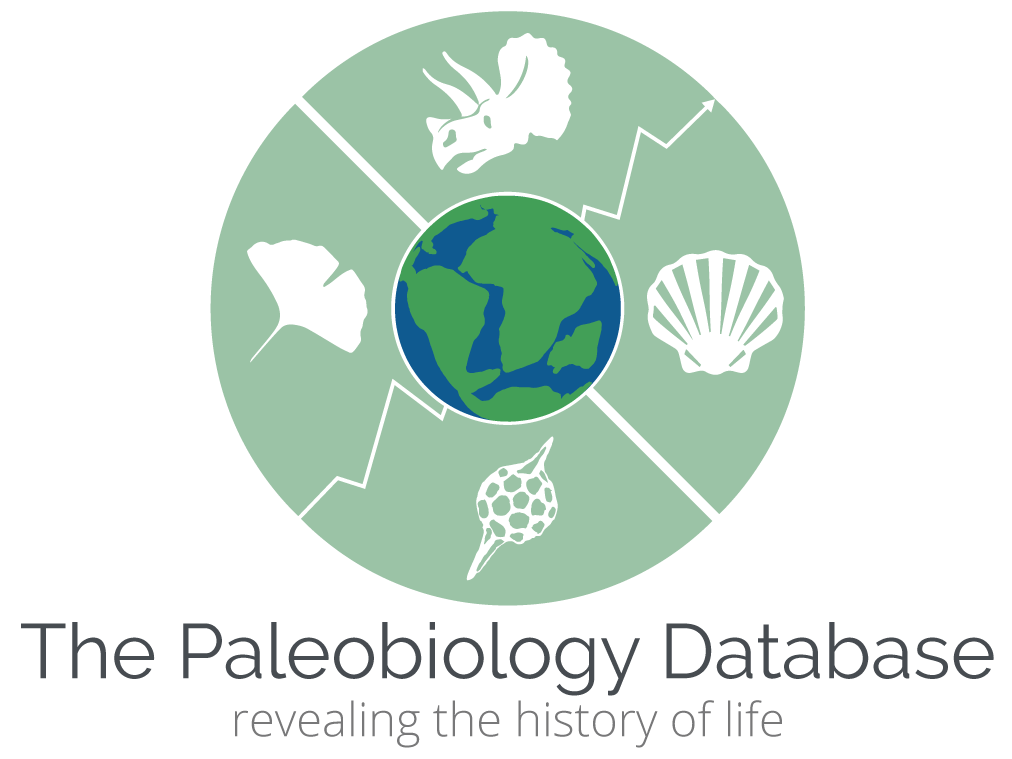
\includegraphics[width=2.75cm,height=2.75cm,keepaspectratio=true]{figure/paleodb}
  \hspace*{0.35\paperwidth}
  
\includegraphics[width=2cm,height=2cm,keepaspectratio=true]{figure/chicago}
}
\date{}

\begin{document}

\begin{frame}
  \maketitle
\end{frame}


\begin{frame}
  \begin{alertblock}{Question}
    When are certain ecologies/ecotypes enriched or depleted?
  \end{alertblock}
\end{frame}

\begin{frame}
  Community structure
\end{frame}

\begin{frame}
  Species pool  
\end{frame}

\begin{frame}
  Bambach Eco-cube ideas from paleo
\end{frame}

\begin{frame}
  Fourth-corner modeling
\end{frame}


\begin{frame}
  results from analysis of extinction selectivity and individual level covariates
\end{frame}

\begin{frame}
  group level covariates
\end{frame}

\begin{frame}
  Inference
\end{frame}

% motivation
%   community structure
%     maxent, sdm-s
%   results from analysis of extinction selectivity
%     decrease in extinction risk through time
%     certain ecologies ``favored'' over others
%   climate/environmental change
%     Paleo vs Neo
%     floral phase
%     global temperature
% approach
%   conceptual diagram 
%   data types
%   diagram of model
%     basic vs full
%       basic uses implied presences
%       full uses absences as data
%     note similarity between concept and model
%     this is a key detail that is missing in most analyses
%   inference
%     complexity and time required
%     ADVI vs NUTS
% results
%   given occurrence, probability is of specific ecology
%   effect of group-level covariates
% conclusions and future directions

\begin{frame}
  \frametitle{Posterior predictive performance}

  \begin{center}
    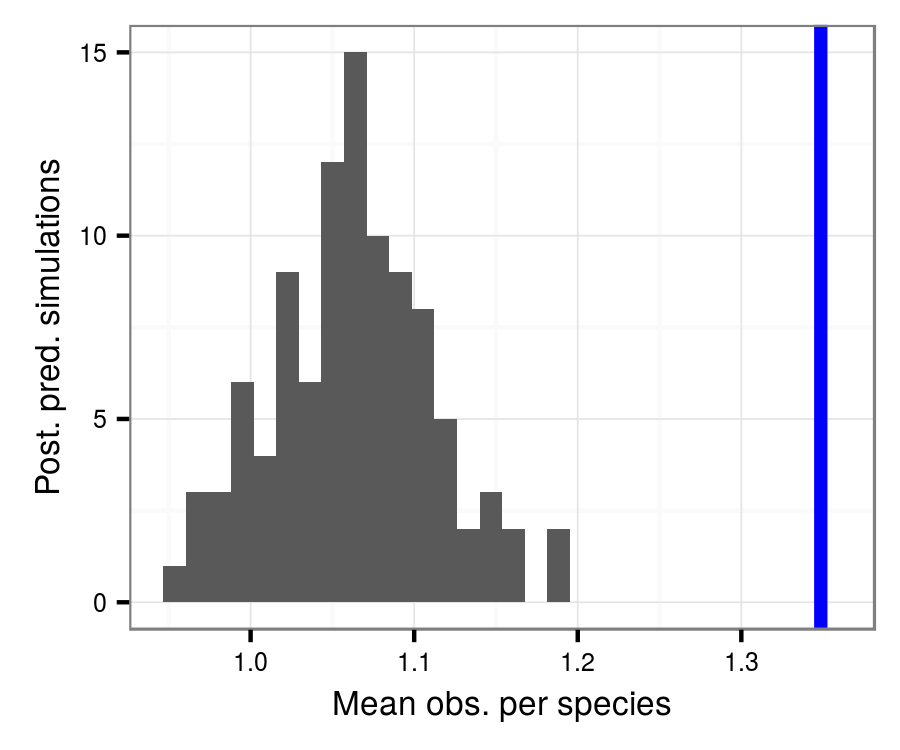
\includegraphics[height=\textheight,width=\textwidth,keepaspectratio=true]{figure/pred_occ}
  \end{center}
\end{frame}


\begin{frame}
  \frametitle{Effect of mass on log-odds of occurrence}

  \begin{columns}
    \begin{column}{0.5\textwidth}
      Basic model

      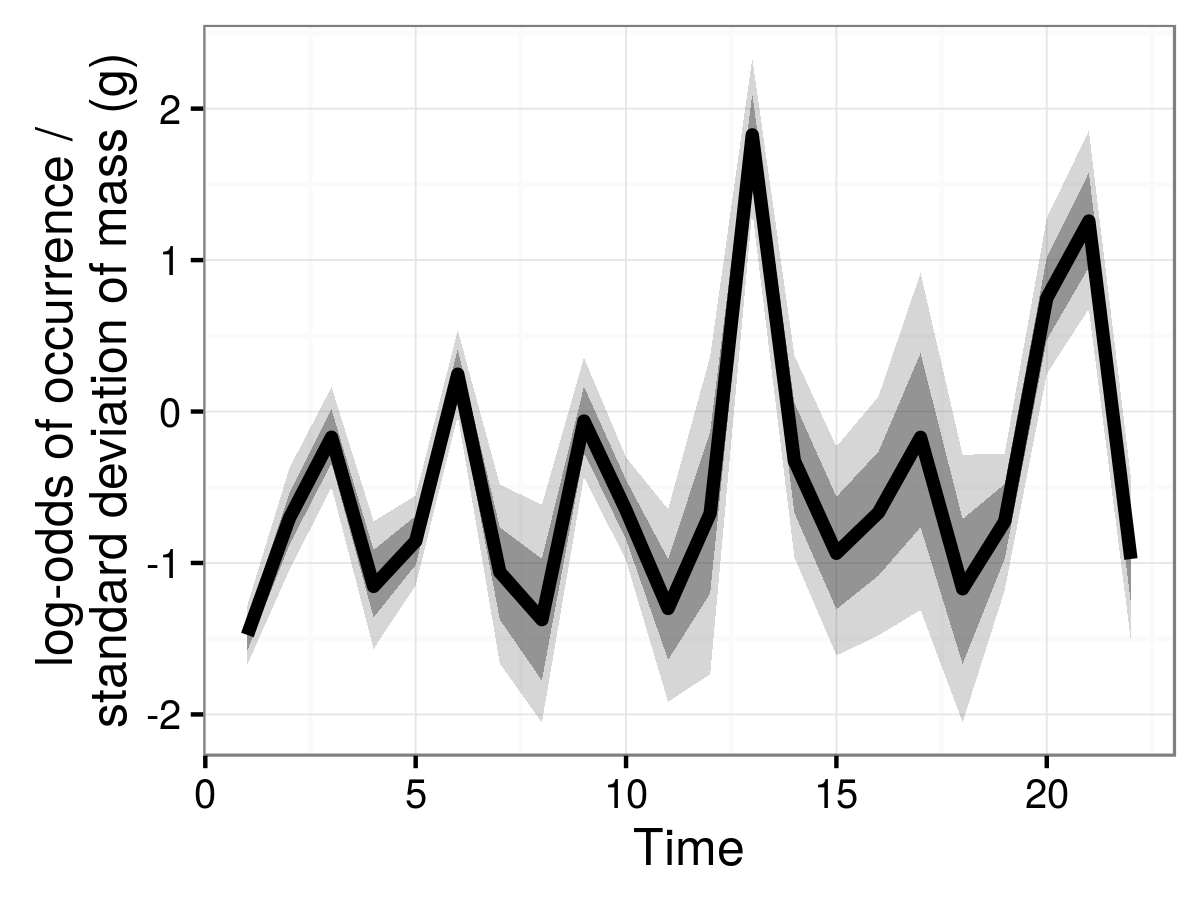
\includegraphics[height=\textheight,width=\textwidth,keepaspectratio=true]{figure/mass_eff_basic}
    \end{column}
    \begin{column}{0.5\textwidth}
      Full model

      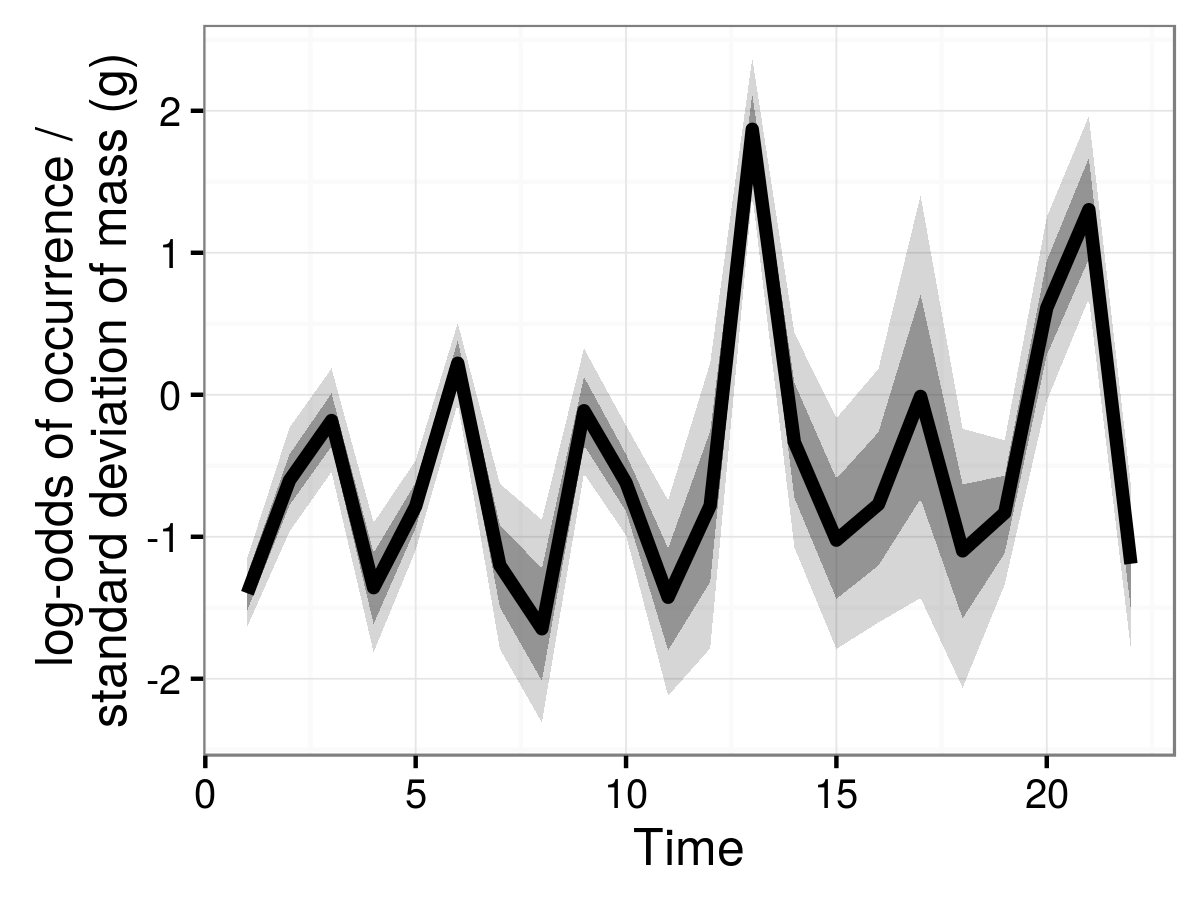
\includegraphics[height=\textheight,width=\textwidth,keepaspectratio=true]{figure/mass_eff_full}
    \end{column}
  \end{columns}
\end{frame}


\begin{frame}
  \frametitle{Probability occurrence is of ecotype (basic model)}

  \begin{center}
    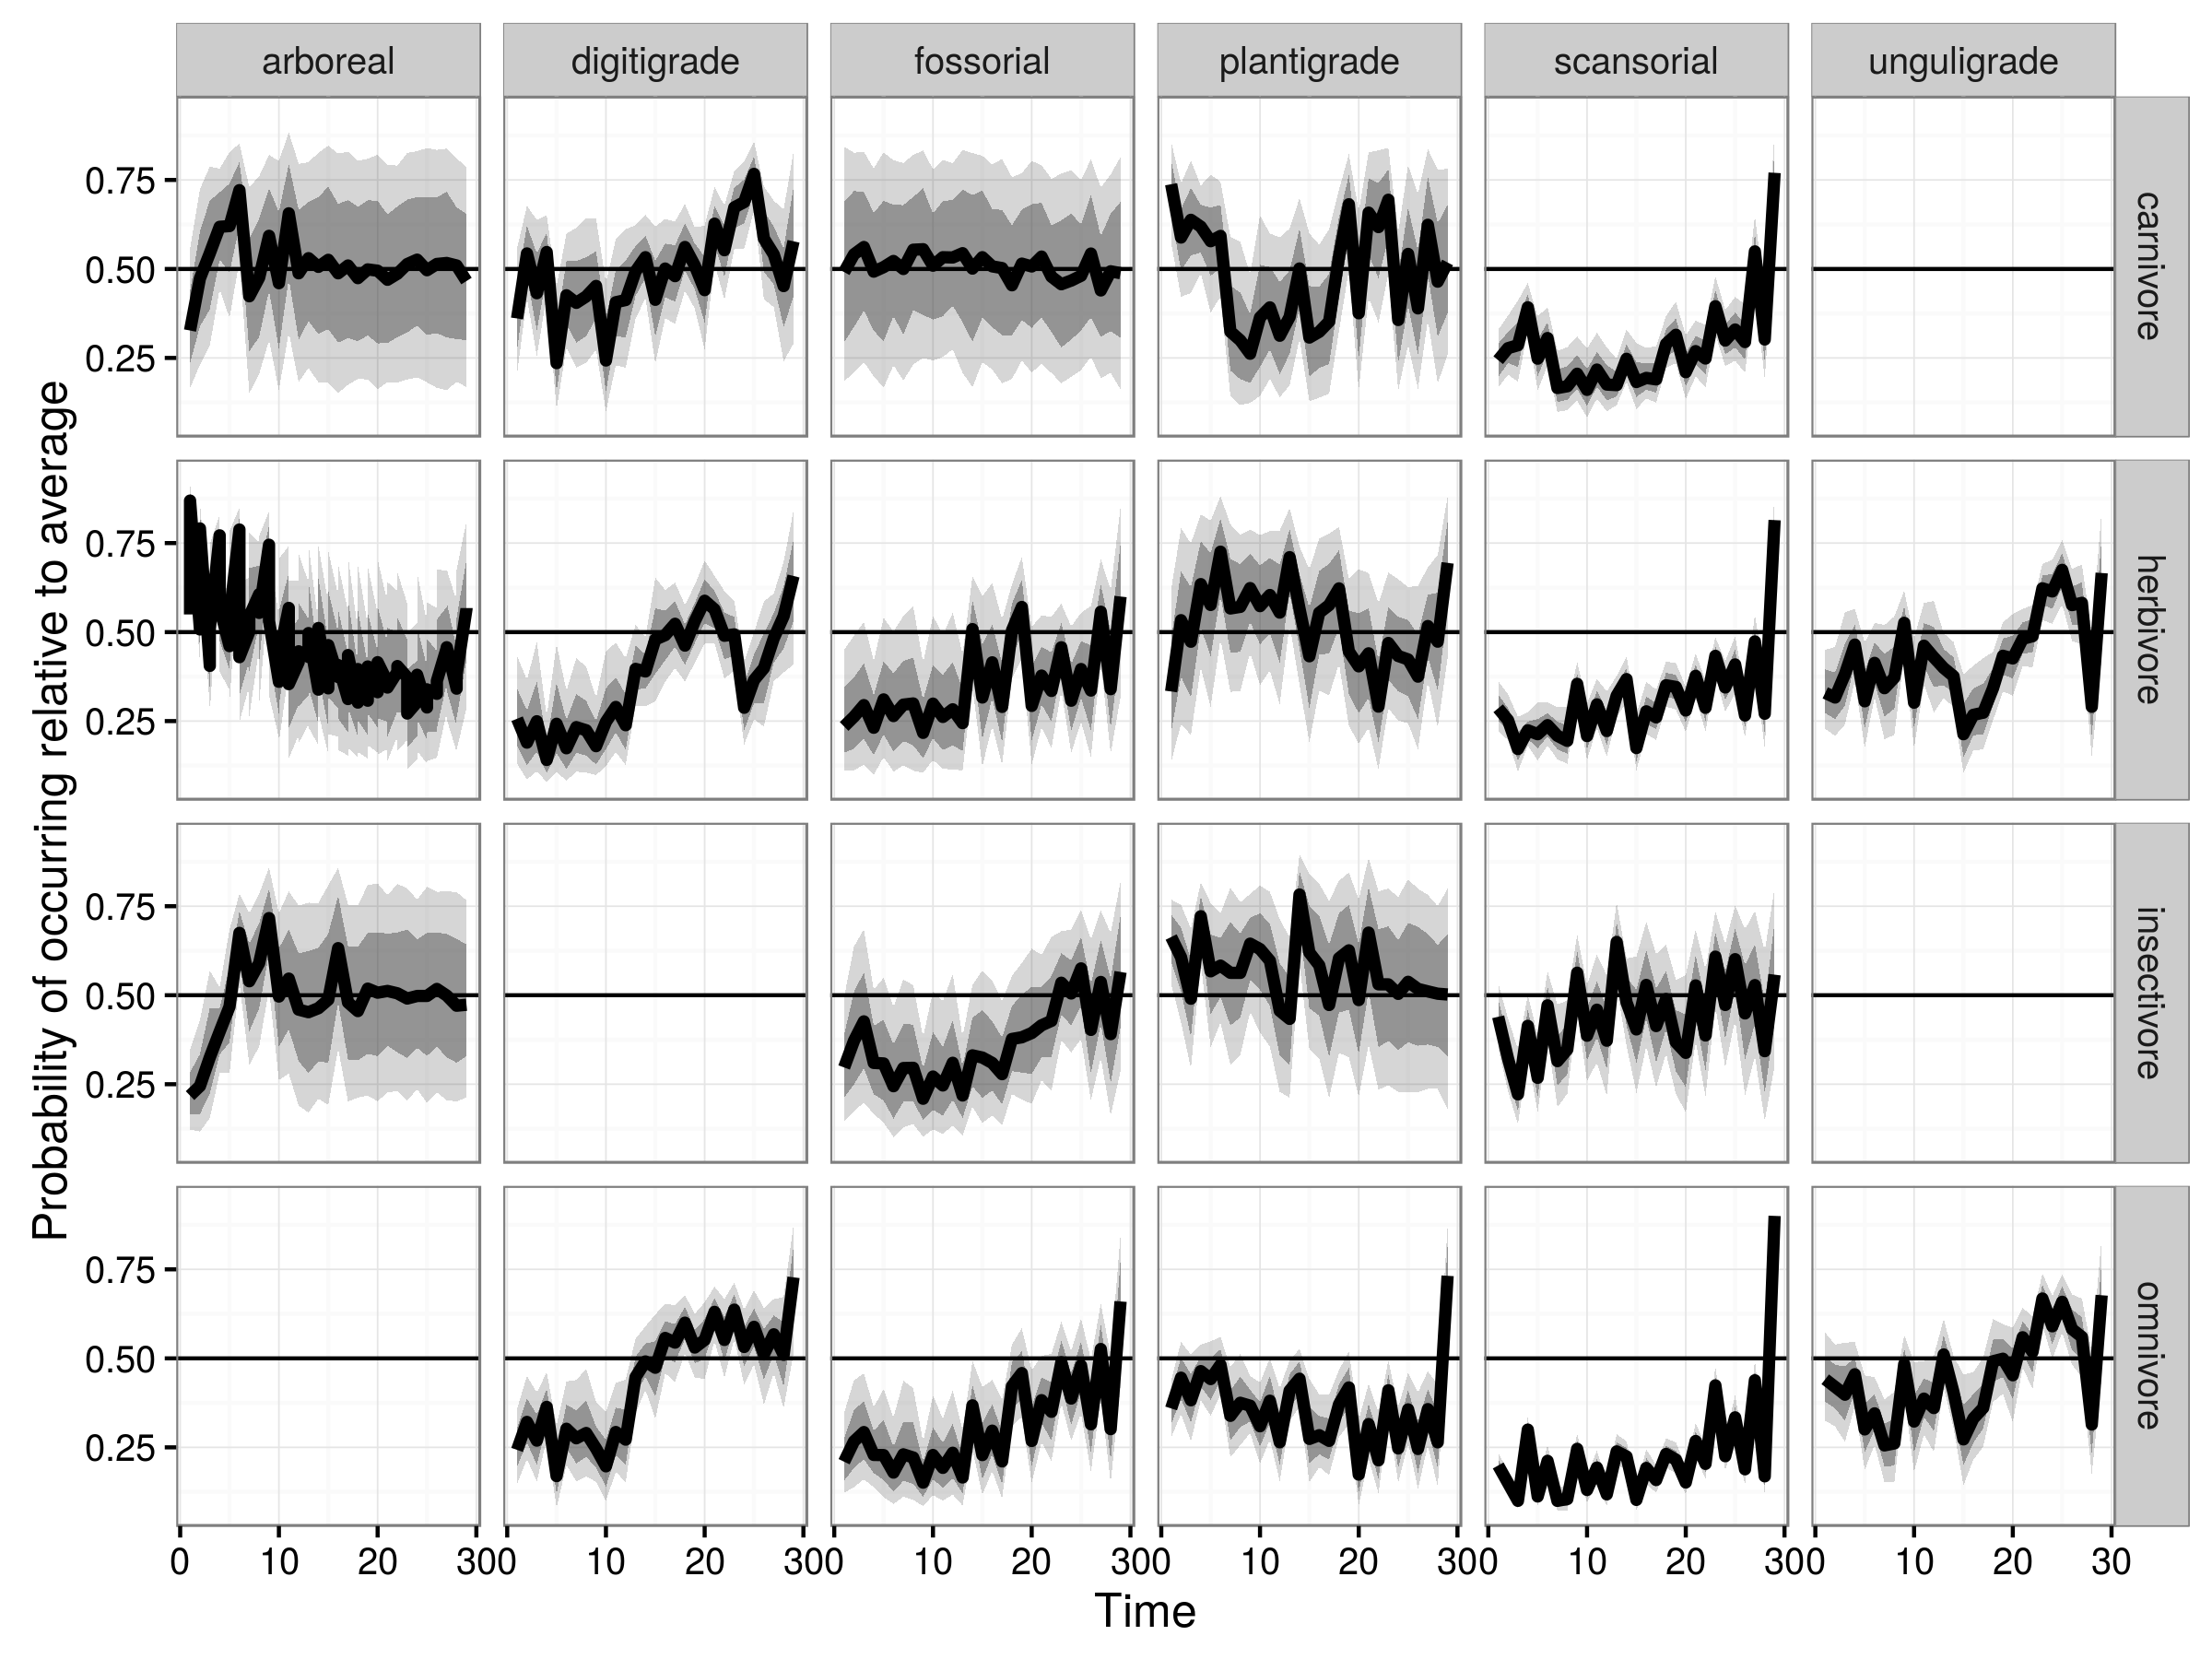
\includegraphics[height=0.8\textheight,width=\textwidth,keepaspectratio=true]{figure/cept_occur_prob_basic}
  \end{center}
\end{frame}

\begin{frame}
  \frametitle{Probability occurrence is of ecotype (full model)}

  \begin{center}
    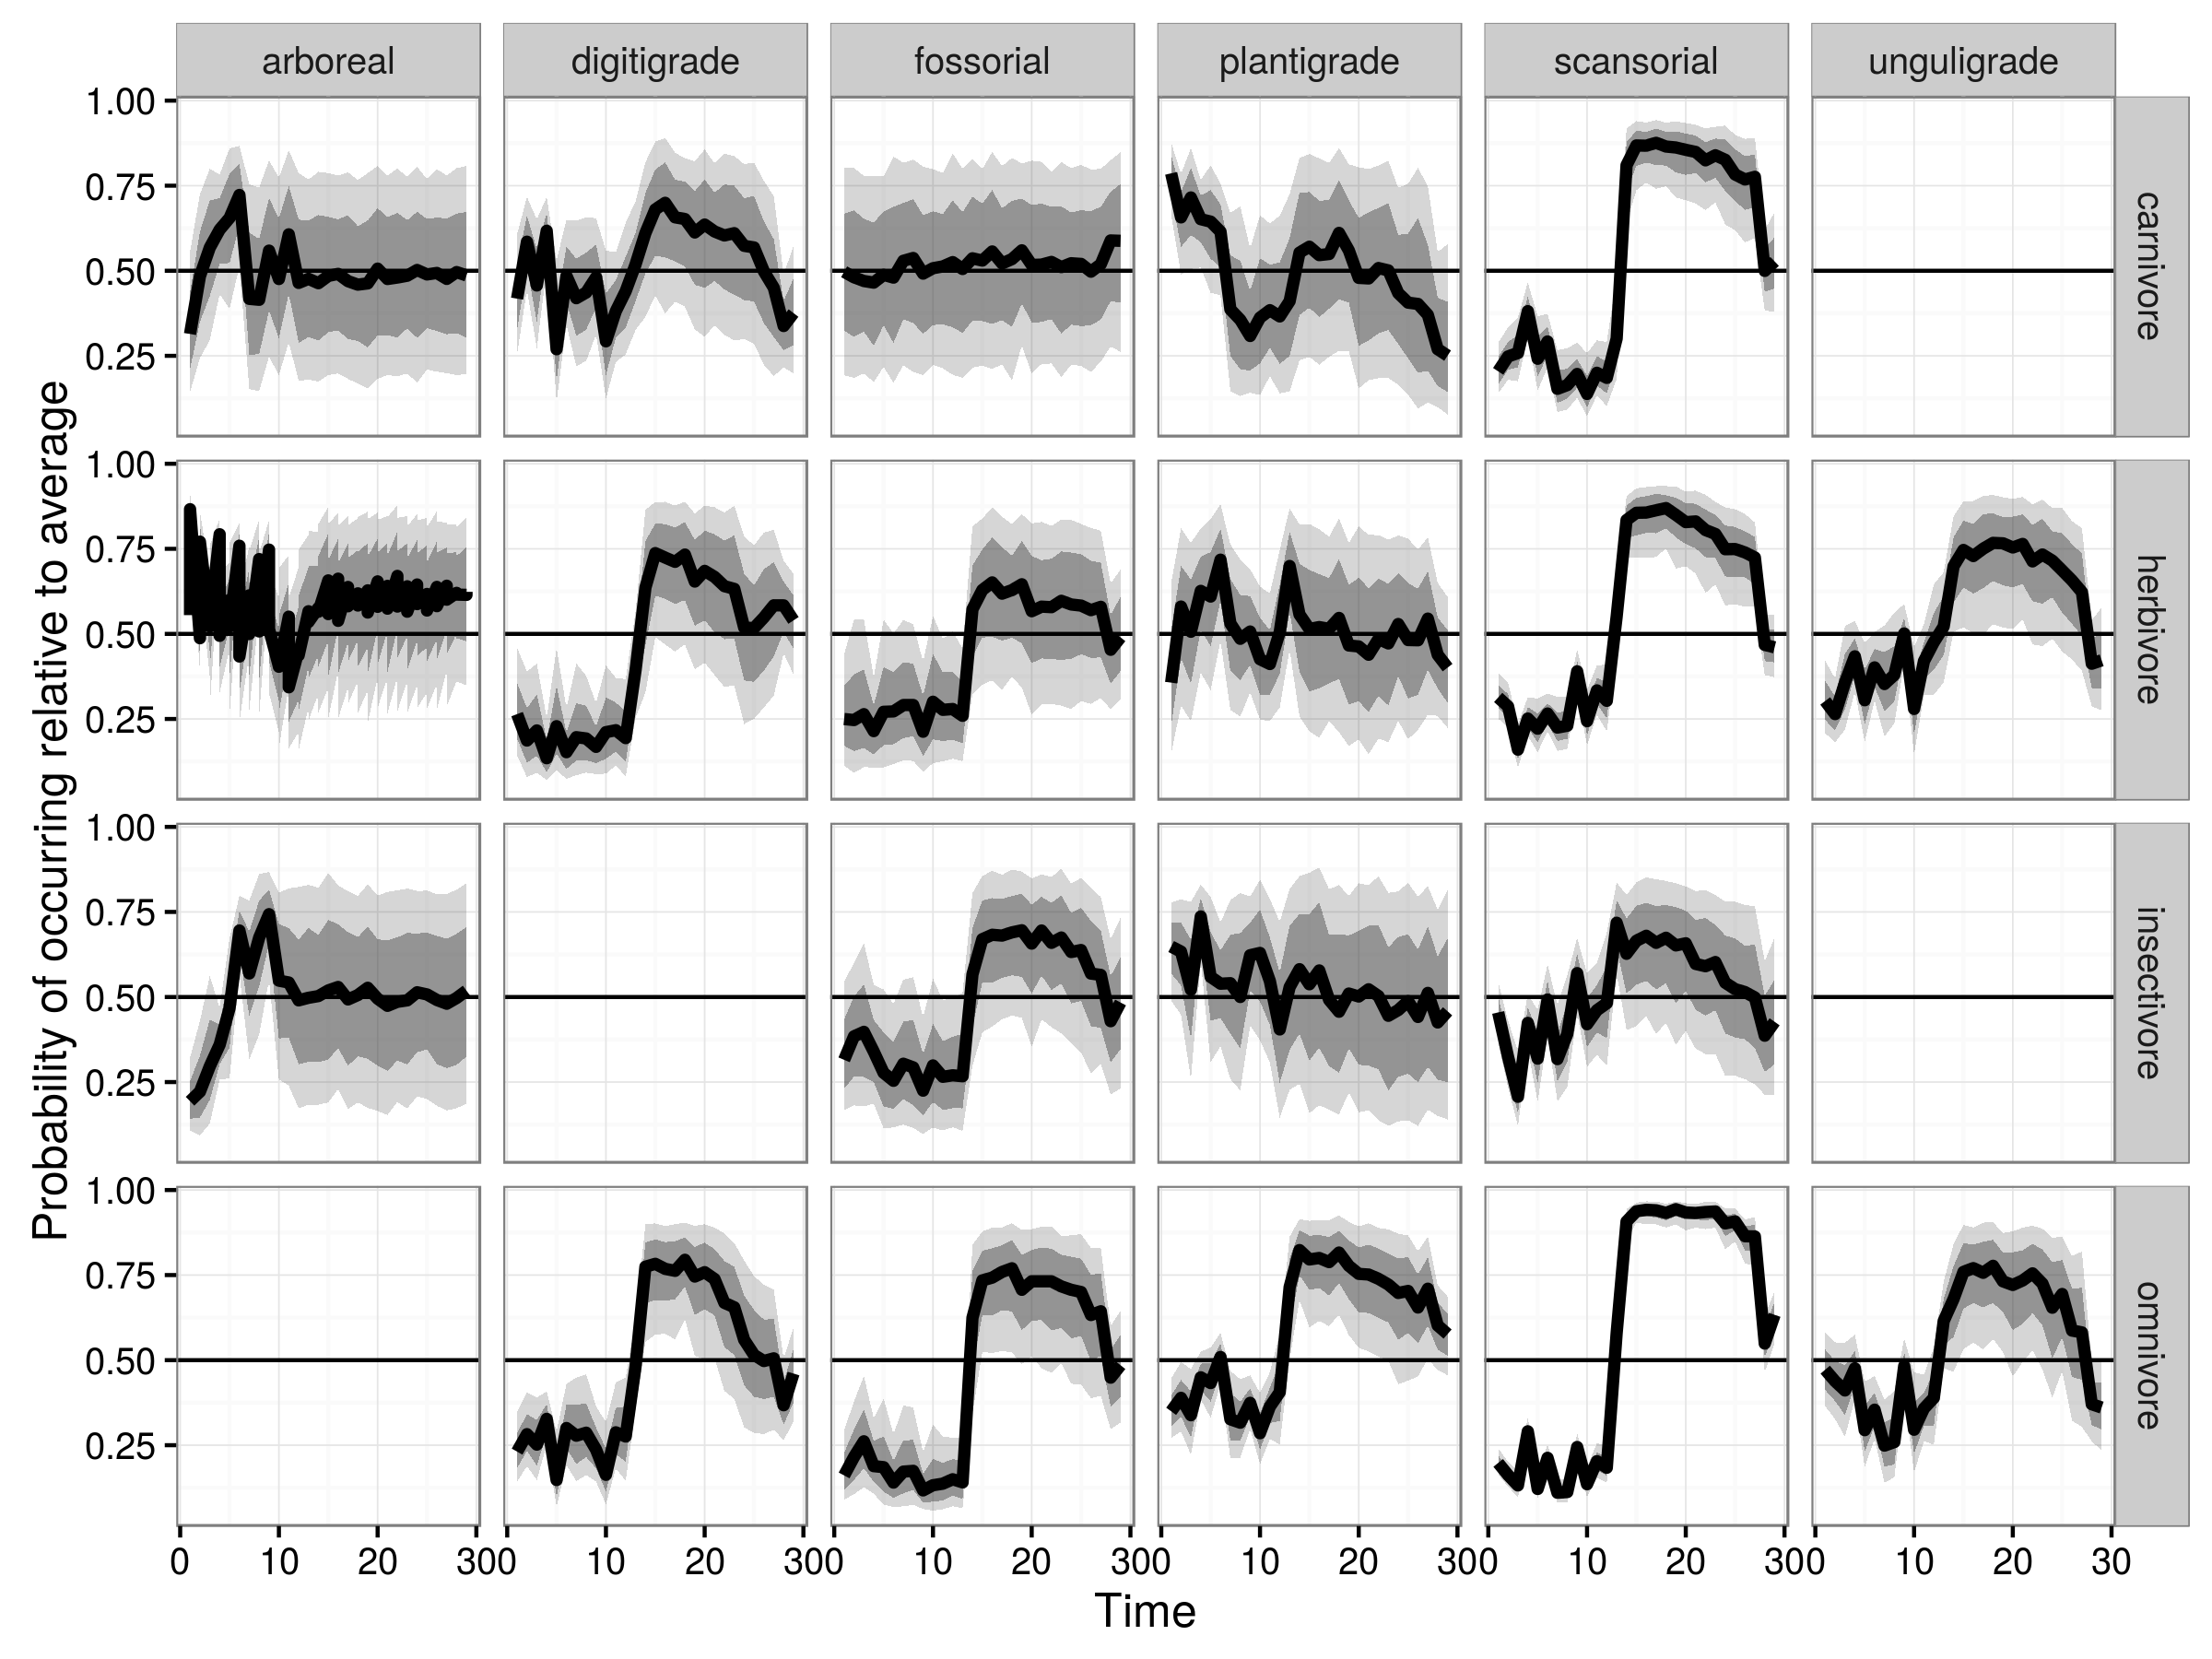
\includegraphics[height=0.8\textheight,width=\textwidth,keepaspectratio=true]{figure/cept_occur_prob_full}
  \end{center}
\end{frame}

\begin{frame}
  \frametitle{Group-level effects (climate, plant phase)}

  \begin{center}
    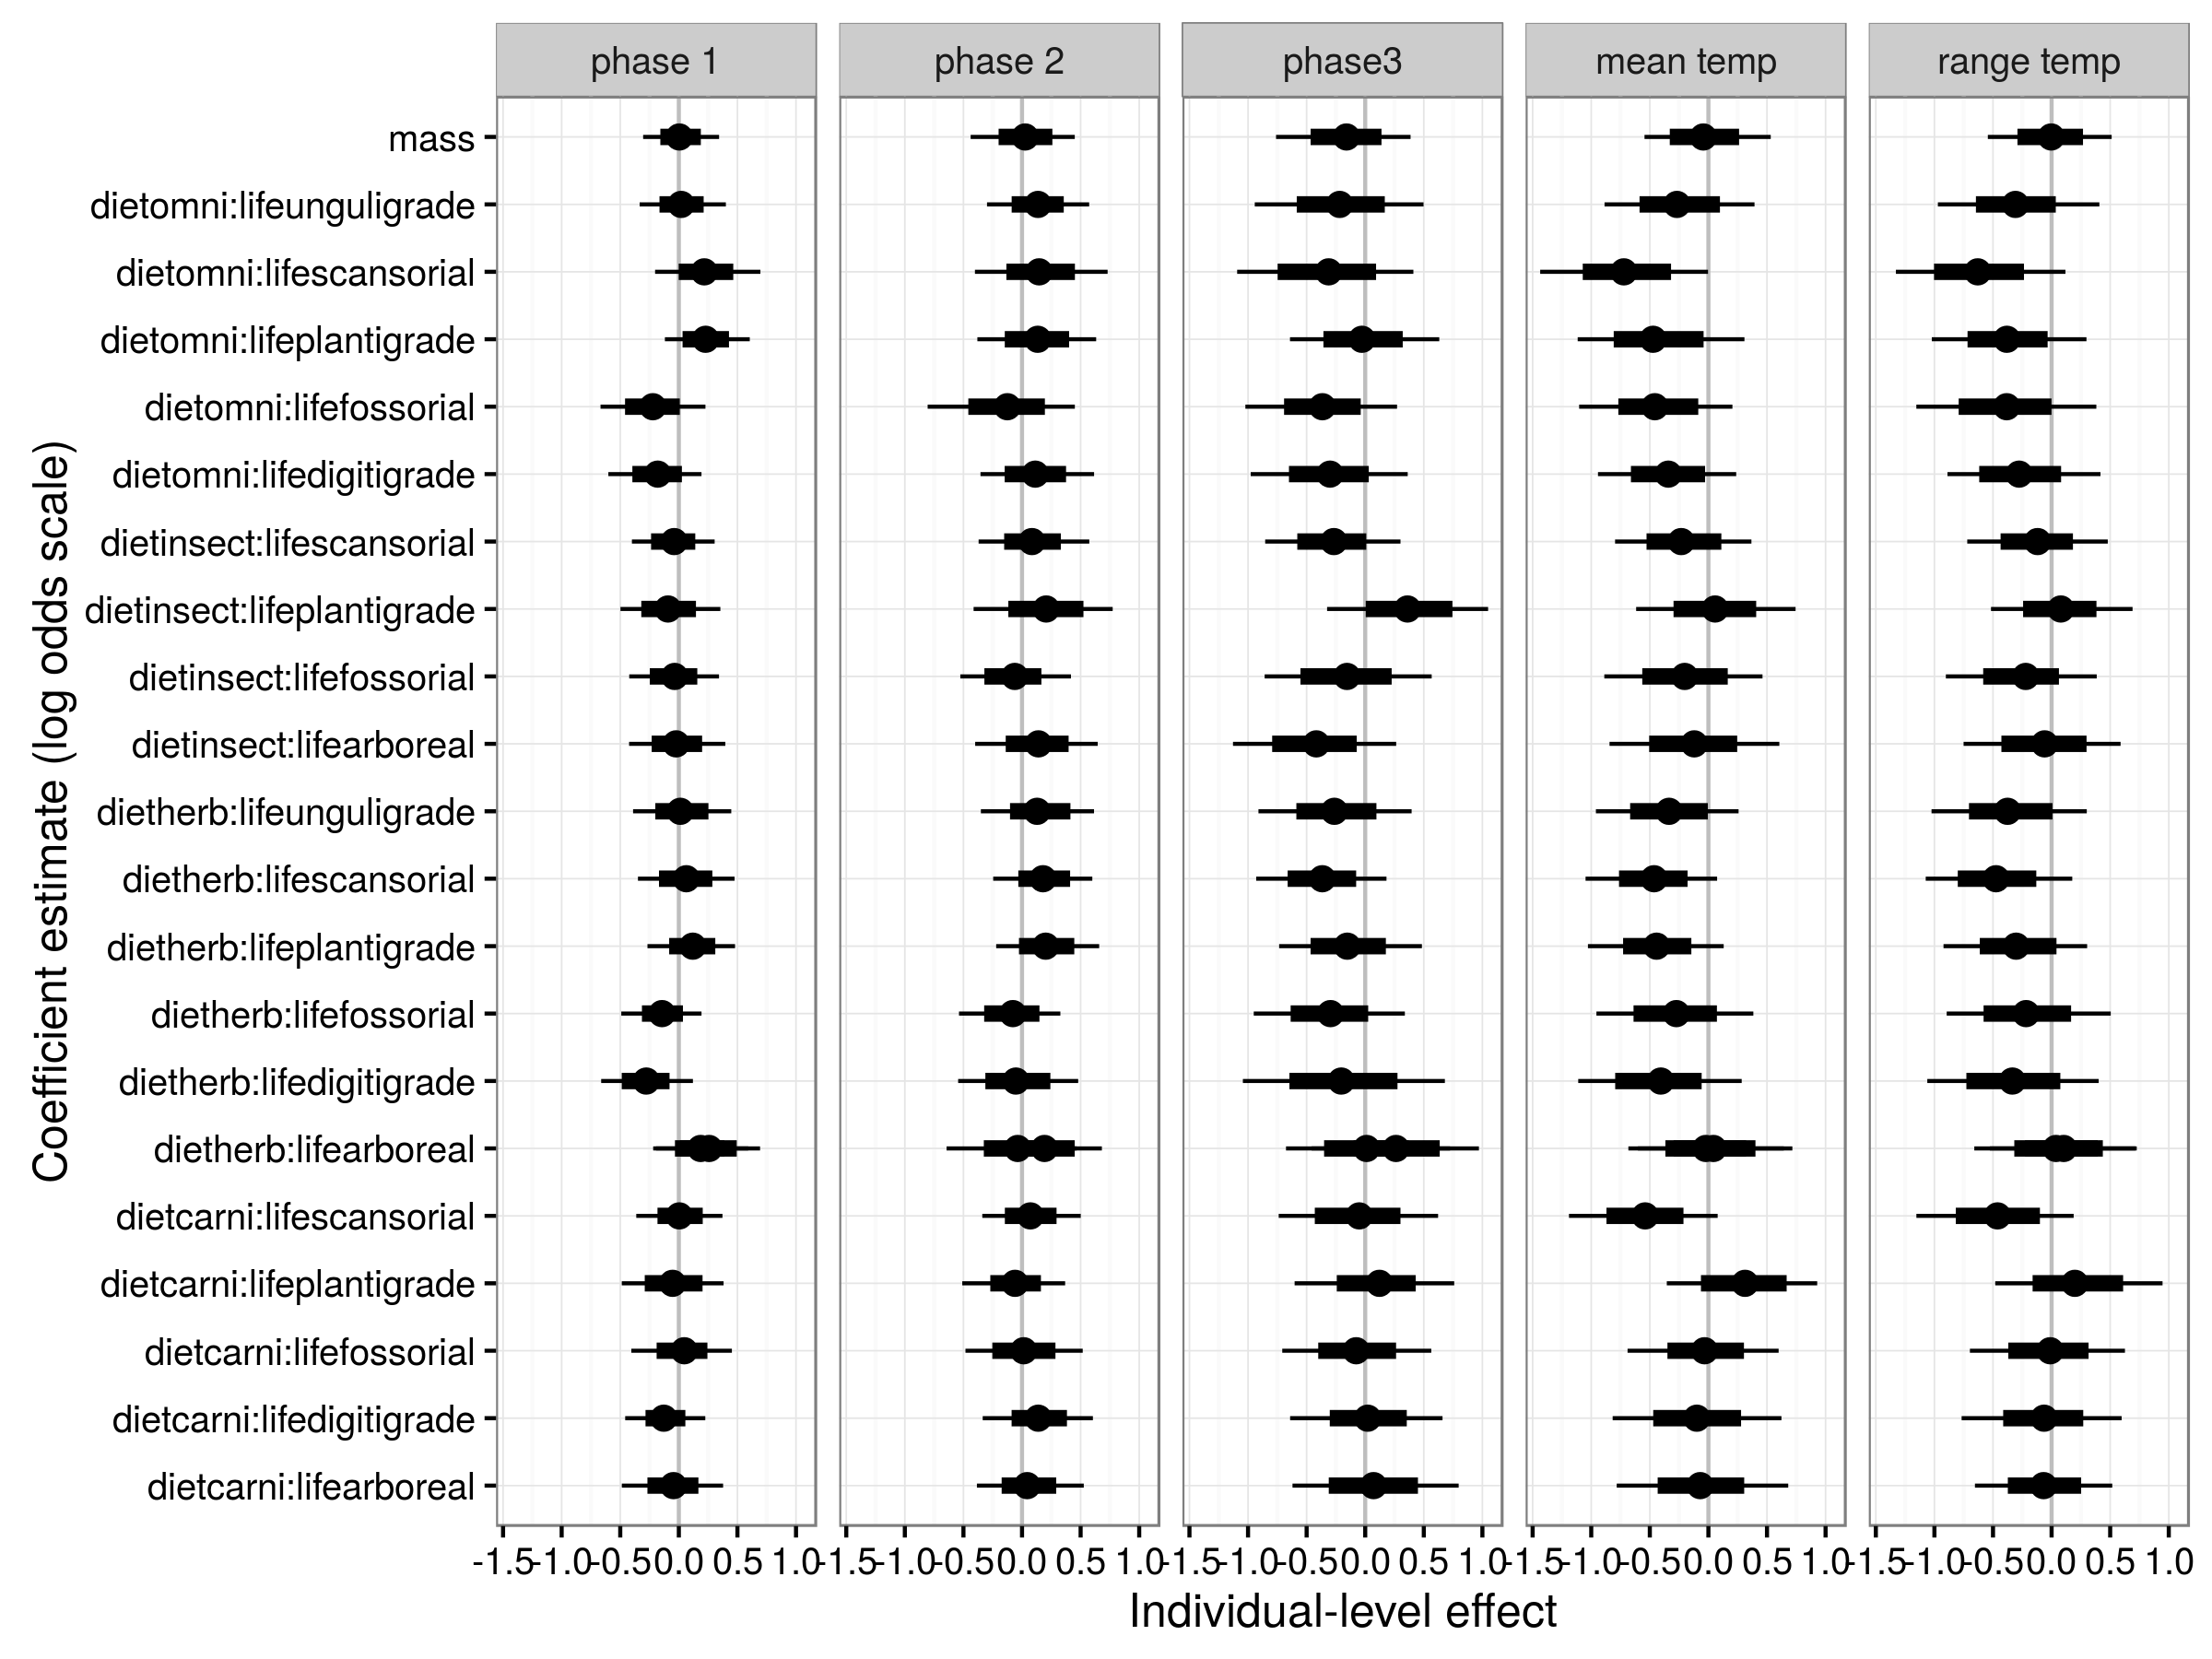
\includegraphics[height=0.8\textheight,width=\textwidth,keepaspectratio=true]{figure/gamma_est_full}
  \end{center}
\end{frame}

\begin{frame}
  \frametitle{Concerns}
\end{frame}

\begin{frame}
  \frametitle{Conclusions}
\end{frame}

\begin{frame}
  \frametitle{Acknowledgements}
\end{frame}



\end{document}
